\documentclass[11pt, twoside]{report}
\usepackage[utf8]{inputenc}
\usepackage[margin=2.5cm]{geometry}
\usepackage{graphicx}  		% display images
\usepackage{rotating}
\usepackage{tikz} 
\usepackage[portuguese]{babel}
\usepackage{indentfirst}
\usepackage[colorlinks=true,linkcolor=black,urlcolor=black,bookmarksopen=true]{hyperref} % Make hyperlinks in index
\usepackage{bookmark} 		% Bookmarks for pdf file
\usepackage{float} 			% colocar as imegens e tabelas dentro do texto
\usepackage{fancyhdr}
\pagestyle{fancy}
\usepackage{tabularx} 		% x column in table can jump a line
\usepackage{setspace} 		% espçamento entre linhas
\usepackage{fancyhdr} 		% creates fancy footers and headers
\raggedbottom				% makes bottom of page more empy to make sure previous text doesnt have vertical gaps
\usepackage{ltablex}
\usepackage{pdflscape}
\usepackage{multirow}
\pagestyle{fancy}
\lfoot{{\footnotesize Tecnologias de Informação}}
\rfoot{{\footnotesize ESTGA}}
\rhead{PTDW}
\lfoot{Calendário de exames}


\renewcommand{\footrulewidth}{1pt}%criar uma linha no que separa o rodapé
%\usepackage{appendix}
%\noindent %sem indentação
%\newcommand{\annexname}{Anexo}
%\makeatletter % treat @ as a letter instead of a control word.
%
%\newcommand\annex{\par
%	\setcounter{chapter}{0}
%	\setcounter{section}{0}
%	\renewcommand\appendixname{Anexo}
%	\renewcommand\appendixpagename{Anexos}
%	\renewcommand{\appendixtocname}{Anexos}
%	\gdef\@chapapp{\annexname}
%	\gdef\thechapter{\@Roman\c@chapter}
%	\renewcommand{\theHchapter}{\annexname.\thechapter}
%	\addappheadtotoc
%}\makeatother



\begin{document}
	
\onehalfspacing % espaçamento de 1,5 entre linhas

	
%	\lhead{Escola Superior de Tecnologia e Gestão de Águeda\\
%		Licenciatura em Tecnologias da Informação
%	}
	
	%\rhead{Capítulo \thechapter}
	\pagenumbering{roman}
	
	\begin{titlepage}
		\centering
		\scshape\Huge Calendário Exames\par
		\vspace{0.9cm}
		
		\scshape\large Projeto Temático em Desenvolvimento Web \\
		\vspace{0.3cm}
		\scshape\large 1º semestre de 2021/2022\par
		\vspace{0.4cm}
		\centering
		%\includegraphics[width=10cm]{}\par
		
		\vspace{1cm}
		
		\large
		Autores\\
		Gonçalo Tavares, Nº 92382  \\
		Bruno Lopes, Nº 86217 \\
		Leonardo Silva, Nº 95381 \\
		Ricardo Fernandes, Nº 49880 \\
		Sofia Rocha, Nº 99991 \\
		
		\vspace{1cm}
		
		\centering
		
\includegraphics[width=10cm]{image/AssB_vertical_cor.png}
		
		\newpage
		\thispagestyle{plain}%retira cabeçalho e rodape
		\thispagestyle{empty}%retira a numeração da pagina
		\centering
		\scshape\Huge Calendário Exames \par
		\vspace{1cm}
		
		\scshape\large Projeto Temático em Desenvolvimento Web\par
		\vspace{1cm}
		\scshape\large 1º semestre de 2021/2022\par
		\vspace{4cm}
		
		
		
		\large
		Autores\\
		Bruno Lopes, Nº 86217 \\
		Gonçalo Tavares, Nº 92382  \\
		Leonardo Silva, Nº 95381 \\
		Ricardo Fernandes, Nº 49880  \\
		Sofia Rocha, Nº 99991 \\
		
		\vspace{1cm}
		Orientadores\\
		Rita Santos \\
		Fábio Marques\\
		\vspace{4cm}
		
		\centering
		
\includegraphics[width=10cm]{image/AssB_vertical_cor}
		
	\end{titlepage}

	\newpage
	\setcounter{page}{1} % começa a contar a paginas no numero 1
	\tableofcontents % Índice de conteúdos
	\thispagestyle{plain} % retira cabeçalho e rodape
	\thispagestyle{empty} % retira a numeração da pagina
	\newpage
	\listoftables % Lista de tabelas
	\newpage
	\listoffigures % Lista de figuras
	
	\newpage
	\pagenumbering{arabic}
	
	\chapter{Introdução}
	
	No âmbito do Projeto Temático em Desenvolvimento Web associado às disciplinas Web Design e Desenvolvimento Web Multiplataforma foi proposto o desenvolvimento de uma Aplicação web para solucionar a necessidade de um cliente. 
	O grupo constituinte deste projecto acordou abordar o tema de gestão de calendários de avaliações que consiste no desenvolvimento de uma página web desenvolvida com as tecnologias web lecionadas no módulo temático que engloba este projecto.
	Este projecto servirá então como solução ao problema apresentado por cliente onde cada funcionalidade será feita à medida mediante as necessidades apresentadas.
	
	Tipicamente quando se pensa num calendário imagina-se um sistema que organize o tempo na forma de anos, subdivididos em meses e por sua vez divididos em dias.
	Este sistema tipicamente usado advém de costumes milenares praticados por várias religiões e civilizações antigas onde a forma mais básica de medir ciclos de tempo vem da observação da rotação do Sol por parte do observador que define um dia, as mudanças da fase da lua que traduz de uma forma bruta o passar de um mês e ainda a observação de estações do ano caracterizadas por eventos climáticos distintos que no seu conjunto formam um ano\cite{stray_mayan_2007}.
	
	Contudo a necessidade de organizar eventos numa escala mais curta de tempo conduz à reorganização de tempo de modo a catalogar acontecimentos associados a pequenos períodos de tempo. 
	A forma sócio-económica mais comum de organizar dias está no uso unitário de horas, ou períodos do dia caso seja essa a necessidade, e estes aparecem representados graficamente numa tabela\cite{10.1145/2702613.2732512} que divide o dia em blocos iguais por forma ao resultado da sua soma ser proporcional \cite{Russell1910-RUSPMV}. 
	Esta forma visual de divisão ajuda a que identificação da duração de um bloco seja facilmente interpretável quando vista de relance. 
	
	Com o avanço da tecnologia no século XX e a popularização do uso da Internet, os calendários tradicionais de papel foram gradualmente caindo em desuso dando lugar a calendário digitais que proporcionam numeras vantagens nomeadamente a portabilidade para todos os tipos de dispositivos modernos, maior complexidade de informação que é permitida armazenar nestes, possibilidade de partilhar calendários e agendas, etc.. 
	
	A organização de calendários digitais contempla várias implementações diferentes cada uma com as suas especificações, formas de implementar e leitura, mas com o evoluir da tecnologia e da criação de standards internacionais, alguns formatos em particular ficara destacados pelo seu uso comum e estandardizado. 
	Destes destaca-se o \textit{Internet Calendaring and Scheduling Core Object Specification} (\textbf{iCal})\cite{rfc2445}, talvez mais conhecido pela extensão de ficheiro comummente partilhado pelos seus utilizadores, "\textbf{.ics}". 
	
	Hoje em dia o simples ato da criação de um calendário ou agenda digital tem em sî concentrado uma vasta panóplia de ferramentas para o fazer, quer seja no uso do calendário de um sistema operativo ou gestor de email que agenda tarefas e notifica antecipadamente, ou numa aplicação para telemóvel que junta a facilidade de uso de \textit{apps} com o design minimalista para a criação de uma agenda rápida ou ainda o uso de páginas \textit{web}, ou \textit{webapps} que pode ser acedido de qualquer dispositivo com capacidade para aceder à Internet. 
	
	De facto existem muitas formas de criar um calendário nos dias modernos, mas do ponto de vista de quem constrói a ferramenta em sî, o princípio é o mesmo, o programador tem sempre de associar uma entidade representativa de um evento a uma hora/data de inicio sendo a duração desta decidida pelo utilizador final. 
	A forma final de apresentação dos resultados ficará no entanto à descrição do cliente/utilizador final que é para este que todo o desenvolvimento de apresentação e funcionalidades é desenvolvido por forma a satisfazer as necessidades.
	Mediante esta realidade a metodologia de trabalho foi baseada em reuniões pré preparadas com o cliente para perceber as necessidades deste, onde retiramos os objectivos principais e identificamos requisitos funcionais e não funcionais.
	São então desenvolvidas soluções baseadas na informação recolhida e posteriormente apresentadas ao cliente inicialmente na forma de protótipos de baixa fidelidade, \textit{wireframes}, e posteriormente versões funcionais de uma aplicação web com intuito de obtenção de \textit{feedback} durante o processo de desenvolvimento.
	
	Este relatório está dividido em vários capítulos começando pela Introdução com uma apresentação breve do evoluir histórico do uso desta ferramenta até às aplicações mais modernas onde se enquadra a solução que será apresentada ao cliente.
	O conjunto de capítulos seguintes serão dedicados ao planeamento do projecto, englobando planeamento do projecto, casos de uso discutidos com o cliente, requisitos funcionais e não funcionais, e casos de utilização.
	Pré implementação está um capítulo dedicado à prototipagem e na implementação irá ser abordado  o modelo de dados persistentes, a implementação e as funcionalidades da aplicação seguido dos testes de funcionamento das mesmas e no final a conclusão.
	
	\section{Objetivos da aplicação}
	
	Este projecto tem como principal objetivo a criação de uma aplicação web para solucionar a necessidade de um cliente que pretende um sistema de criação de calendários digitais para agendamento de um período de avaliações académicas num estabelecimento de ensino superior. 
	Visto o produto final ser projetado para ser distribuído pela comunidade académica, existe também o objectivo principal de exportação num formato facilmente transmissível entre dispositivos.  
	
	Este projecto irá então dedicar-se a satisfazer os seguintes objectivos para a \textit{webapp}: 
	\begin{itemize} 
		\item \textit{Webapp} de fácil navegação e intuitiva para a criação de um calendário. 
		\item Possibilidade de agendamento de exames a unidades curriculares separados por curso, ano letivo e semestre.   
		\item Possibilidade de edição de curso, do docente, unidades curriculares, salas e o seu tipo. 
		\item Exportação de calendários para formato pdf e csv. 
	\end{itemize} 
	\section{Estado de arte}
	
	A partir de uma pequena introdução do tema foi feita uma pesquisa sobre aplicações semelhantes para discutir com o cliente sobre a aplicação a ser criada. A pesquisa resultou em duas aplicações: uma em versão mobile e outra em versão web.
	
	A primeira aplicação, que se chama "Timetable", tem como objetivo organizar todas as aulas, exames e tarefas escolares de um aluno. O utilizador pode adicionar aulas e exames (ver figura \ref{inserirvizualizaraula}), indicando a sala, o nome da disciplina, a data de início e fim, o nome do docente, o tipo e o dia da semana em que se realiza, sendo diferenciados pela frequência - as aulas são repetidas a cada semana e o exame só se realiza uma vez. Para além disso o aluno pode associar tarefas tanto a aulas como a exames podendo vizualizar estas informações em forma de lista ou em calendário (ver figura \ref{dayweekview}).
		\begin{figure}[H] 
		\centering 
		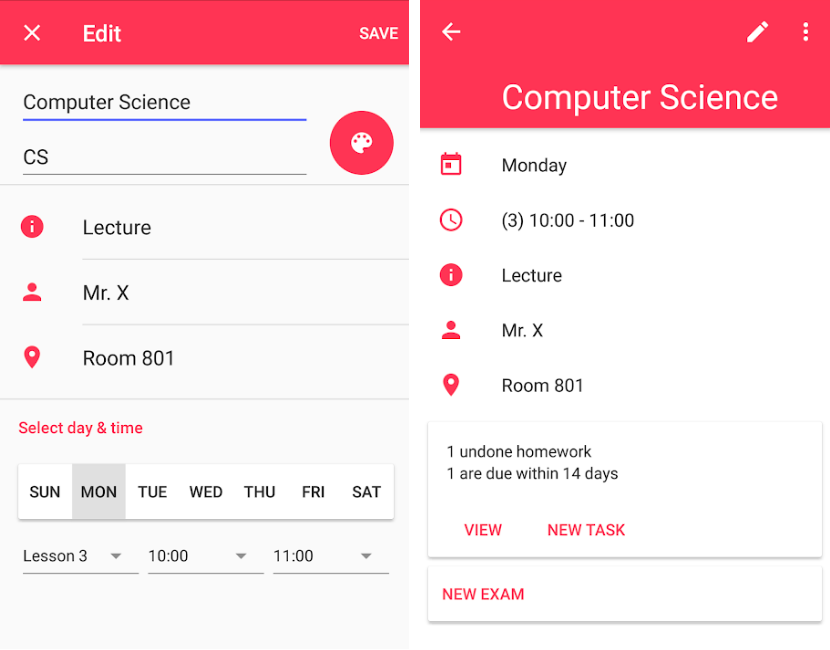
\includegraphics[width=0.7\textwidth,height=0.7\textheight,keepaspectratio]{image/estadodearte/inserirevizualizar}
		\caption{Inserir e vizualizar a aula criada}
		\label{inserirvizualizaraula}
	\end{figure}

	\begin{figure}[H] 
		\centering 
		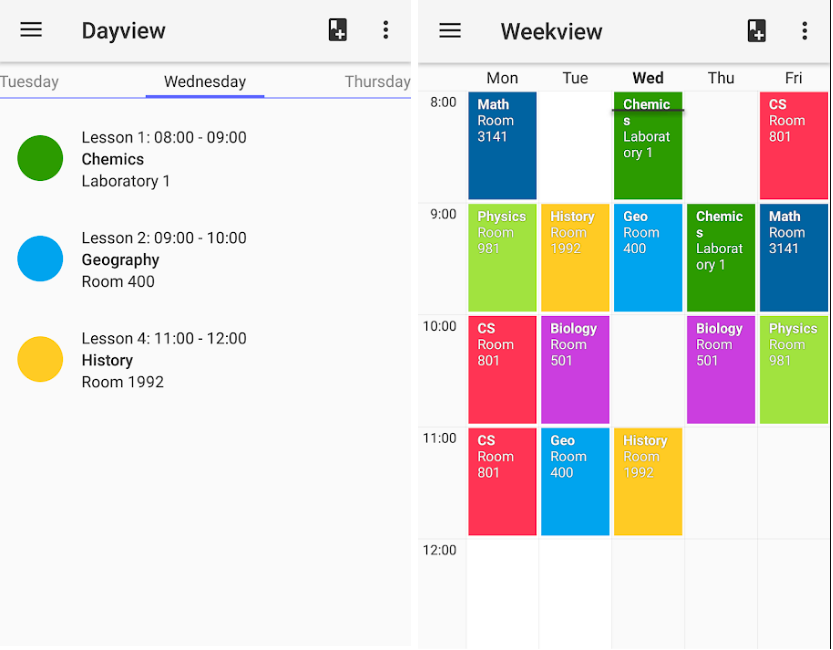
\includegraphics[width=0.7\textwidth,height=0.7\textheight,keepaspectratio]{image/estadodearte/dayweekview}
		\caption{Lista de aulas e o calendário escolar semanal}
		\label{dayweekview}
	\end{figure}

	A segunda aplicação ``StudyLife'' tem o mesmo objetivo que a aplicação anterior no entanto a sua apresentação gráfica é diferente (ver figura \ref{listastudylife}). Poderá criar tarefas e exames associados a disciplinas, previamente criadas. Para cada tarefa pode indicar qual é a sua percentagem de realização (?) e nos exames pode-se vizualizar o dia e a hora do mesmo, a sala, se existe conflitos com aulas ou não e quanto tempo o aluno tem para o realizar, tal como se pode vizualizar na figura \ref{examematematica}. Estas informações podem ser vistas em forma de lista (\ref{listastudylife}) ou em forma de calendário semanal.
	
	
\begin{figure}[H] 
	\centering 
	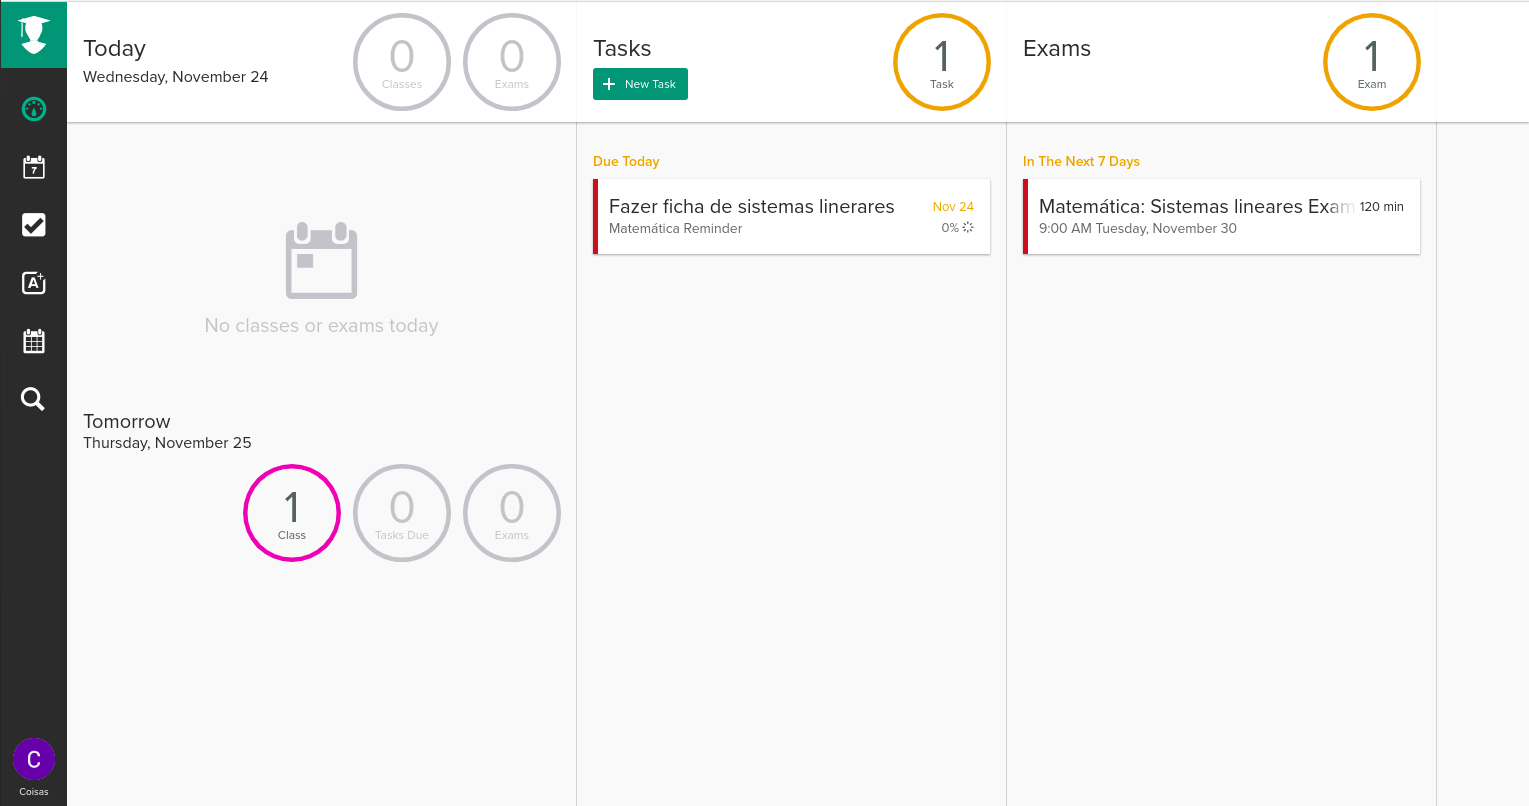
\includegraphics[width=0.8\textwidth,height=0.8\textheight,keepaspectratio]{image/estadodearte/calendario}
	\caption{Lista de tarefas e exames}
	\label{listastudylife}
\end{figure}

\begin{figure}[H] 
	\centering 
	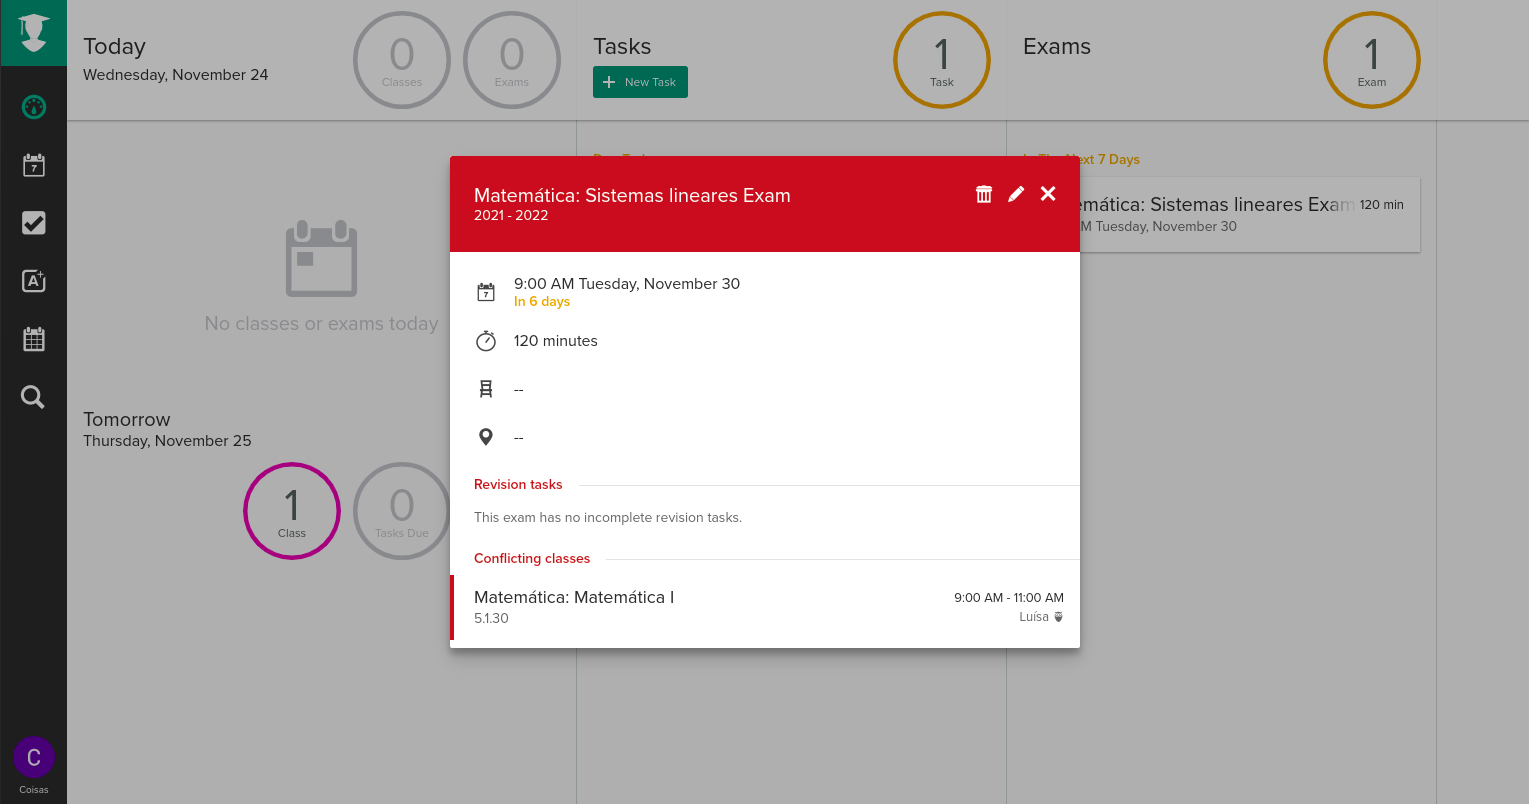
\includegraphics[width=0.8\textwidth,height=0.8\textheight,keepaspectratio]{image/estadodearte/informacoesexame}
	\caption{Visualização de informações sobre o exame de Matemática}
	\label{examematematica}
\end{figure}

\begin{figure}[H] 
	\centering 
	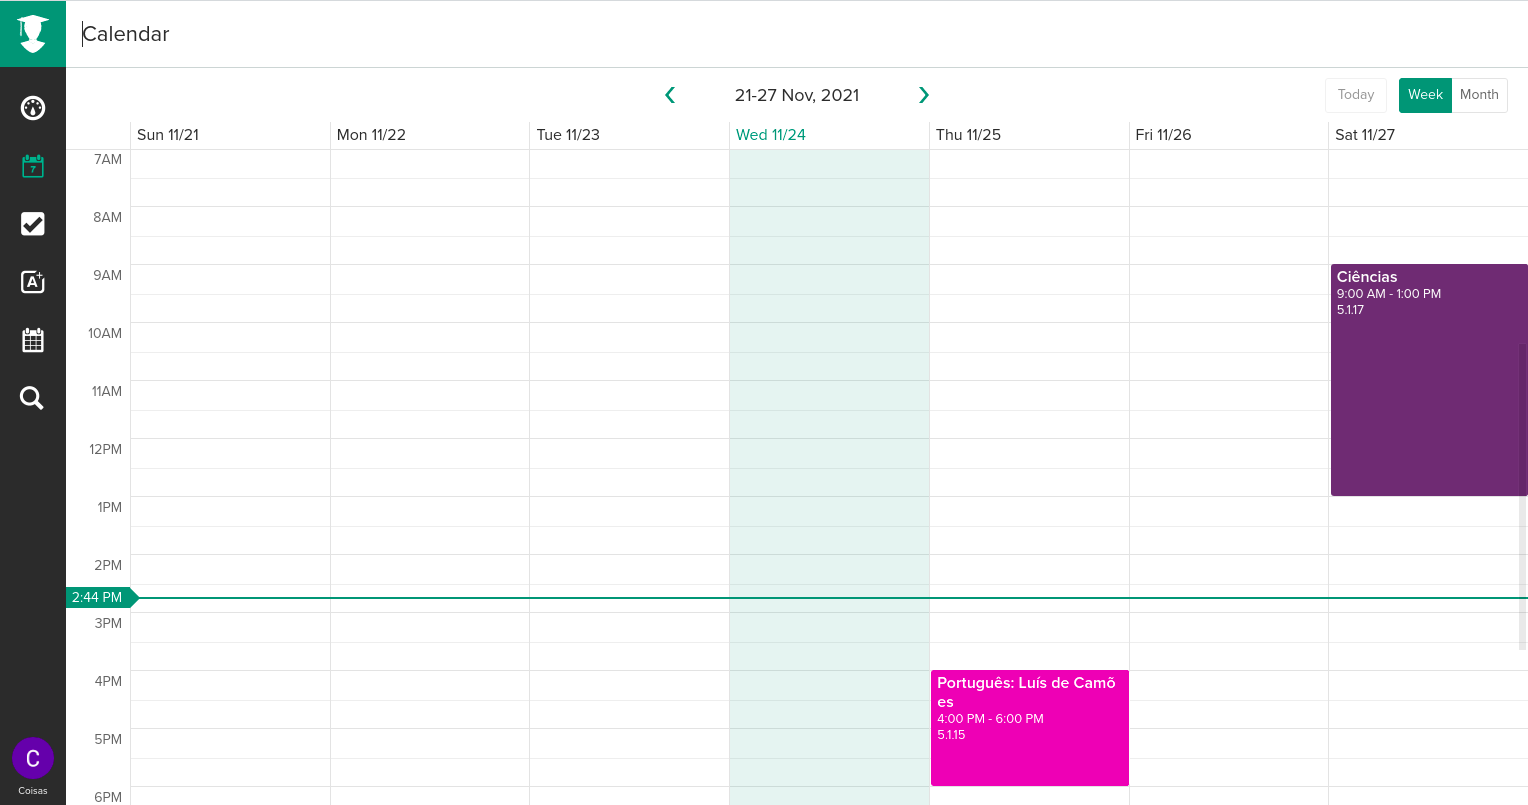
\includegraphics[width=0.8\textwidth,height=0.8\textheight,keepaspectratio]{image/estadodearte/calendariostudy}
	\caption{Visualização de informações em forma de calendário semanal}
	\label{calendariostudylife}
\end{figure}




	 
	
	
	\chapter{Planificação do projeto}

 	
		
	\clearpage
	\begin{landscape}
		\pagestyle{empty}
		
		\begin{figure}[H] 
			\centering 			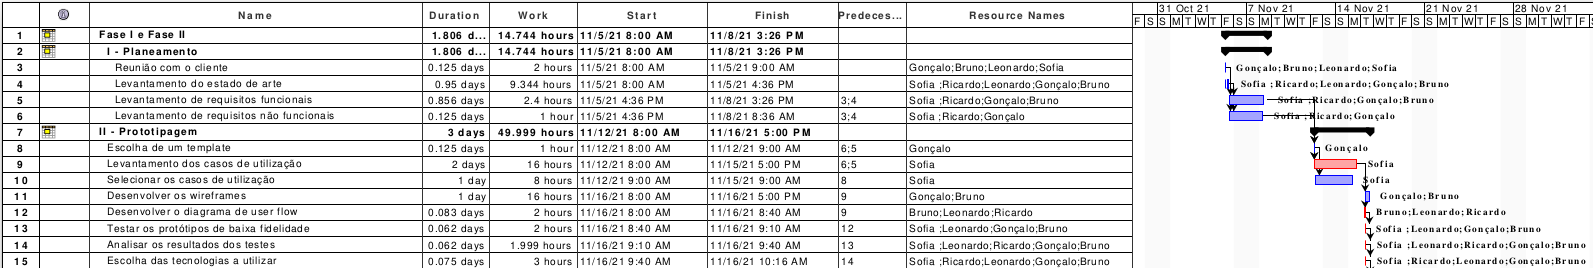
\includegraphics[width=1.4\textwidth,height=1.4\textheight,keepaspectratio]{image/planeamento_1fase}
			\caption{Planeamento da primeira e segunda fase}
			
		\end{figure}
	\end{landscape}
	
	
	\chapter{Análises dos utilizadores e tarefas}
	
	Após a primeira renuião com o cliente chegou-se à conclusão que  este é também um potencial utilizador e que tem uma ideia precisa das funcionalidades da aplicação. Por isso, aliado à restrição de tempo achou-se que não se iria aprofundar na análise dos utilizadores. 
	
	O cliente no momento recorre ao excel para a criação de calendários,  colocando todas as salas, cursos e etc com alto risco de erro e com baixa eficiência. Para além disso a formatação final (em .pdf) é exportado a partir do excel.

	
	



	processo atual da criação dos calendários de exames
	reunião com o cliente
	
	\chapter{Modelo de requisitos}
	\section{Requisitos funcionais}
	
	
	Os requisitos funcionais representam todas as funcionalidades que o sistema pode fazer ou que o utilizador pode realizar no sistema. Com isso na tabela \ref{requisitiosfuncionais} estam todos os requisitos funcionais dividos por várias categorias: importação, exportação, marcação de exames, configurações, avisos, pesquisa e outros (requisitos que não se encaixam em nenhuma das categorias descritas). Dentro da categoria "avisos" tem as funcionalidades que o sistema irá realizar após uma ação do utilizador, ao contrário de todas as outras categorias em que o utilizador tem a possibilidade realizar determinada tarefa.
	
	Para além disso os requisitos funcionais estam classificados por prioridade sendo os de alta prioridade realizados nas primeiras fases e os de baixa prioridade implementados nas últimas fases (ver secção \ref{selecaocasosdeuso}).  
	
	
	
\def\arraystretch{1.5}%
	\begin{center}
		\label{requisitiosfuncionais}
		\begin{longtable}{|m{1cm}|m{2.2cm}|m{10cm}|m{2cm}|}
			\caption{Requisitos funcionais}\\
			
			\hline			
			\textbf{Refª }	& \textbf{Categoria}&\textbf{Descrição do requisito} & \textbf{Prioridade} \\
			\hline
			
			
			RF.1 &Importação& Importação de ficheiros com a configuração de salas, disciplinas e docentes em formato .csv & Alta \\
			\hline
			
			RF.2 &\multirow{2}{2cm}{Exportação}& Exportação de calendários em formato .pdf & Alta \\
			
			RF.3 && Exportação o calendário em língua Inglesa & Baixa \\
			\hline
			
			RF.4 &\multirow{3}{2cm}{Marcação de exames}& Os exames podem ser marcados em três turnos: manhã (às 9h30), tarde (às 14h) e noite (às 18h30) por padrão & Alta \\
			
			RF.5 && O utilizador pode associar vigilantes a cada exame & Alta \\
			
			RF.6 && Criação épocas de avaliação adicionando um nome e uma data de início e fim & Alta \\
			
			RF.7 && O calendário não deverá permitir a marcação de exames aos domingos e feriados & Alta \\
			RF.8 &&O utilizador pode associar a cada exame vários vigilantes & Alta\\
			
			RF.9 &&	O utilizador pode associar mais do que uma sala a um exame & Alta\\
			
			RF.10 && Se houver vários cursos com o mesmo exame então será associado a todos os calendários dos cursos associados. & Média\\
			\hline
		
			RF.11. &\multirow{6}{2cm}{Configurações}& Configurar tipo de sala com equipamento e lotação total & Alta \\
			
			RF.12. & 	& Inserção de cursos e disciplinas & Alta\\
			
			RF.13. && Permitir inserir novos docentes & Alta\\
			
			RF.14. && Permitir editar informações (nome, que disciplinas está a lecionar, horário de trabalho) sobre os docentes & Alta\\
			
			RF.15. && Permitir colocar restrições arbitrárias introduzidas pelo utilizador & Baixa \\
			
			RF.16. && Permitir associar na área do docente dias em que os mesmos não estão disponíveis & Alta\\
			
			\hline
			
			RF.17 &\multirow{9}{2cm}{Avisos}& Aparecimento de um aviso no caso de incongruência da informação durante a marcação de exames & Alta \\
			
			RF.18 &&Mostrar um aviso de alta prioridade se houver sobreposições de exames & Alta\\
			
			RF.19 && Mostrar um aviso de alta prioridade se o docente não estiver disponível & Alta \\
			
			RF.20 && Mostrar um aviso de alta prioridade se a sala não estiver disponível & Alta\\
			
			RF.21 && Mostrar um aviso de alta prioridade se o curso for diurno e colocar um exame no turno da noite e vice-versa & Média\\
			
			RF.22&&Mostrar um aviso de alta prioridade se o docente associado ao mesmo exame for repetido & Alta \\
			
			RF.23 && Mostrar um aviso de alta prioridade se o exame necessitar de uma sala de informática e não for associada sala desse tipo & Média\\
			
			RF.24 && Mostrar um aviso de alta prioridade se houver mais alunos inscritos do que  lotação máxima da sala & Alta\\
			
			RF.25 && Mostrar um aviso de média prioridade se houver exames marcados no mesmo dia e hora do mesmo curso mas anos diferentes & Média\\
			\hline
			
			RF.26 &Autenticação& O utilizador só pode aceder à aplicação após a autenticação & Alta\\
			\hline
			RF.27 &\multirow{2}{*}{Pesquisa}& O utilizador pode utilizar um ou mais filtros na pesquisa de calendários & Alta\\
		
			RF.28  && Pesquisar por calendários com filtro por cursos, ano, semestre e época de avaliação  & Alta \\
			\hline
			
			RF.29 &\multirow{2}{*}{Outros}& A criação de um novo calendário deverá sempre partir do início sem nenhuma configuração associada & Alta\\
		
			RF.30 && Guardar e visualizar calendários de exames de anos anteriores sem informações específicas (perguntar ao Paulo) & Média \\
			\hline
		\end{longtable}
	\end{center}



	
	\section{Requisitos não funcionais}
	
	Os requisitos não funcionais estam dividos em três categorias: requsitos de interface e facilidade de uso que representam todos os requisitos que melhorem a usabilidade da aplicação; requisitos de segurança e integridade dos dados e requisitos de interface com sistemas externos e ambientes de execução.
	
	\subsection{Requisitos de interface e facilidade de uso}

	
	\begin{table}[H]
	\caption{Requisitos de interface e facilidade de uso}
	
	\begin{center}
		\begin{tabularx}{\textwidth}{|c|X|c|}
			\hline
			\textbf{Refª }	& \textbf{Descrição do requisito} & \textbf{Prioridade} \\
			\hline
			RIF1 & As disciplinas e cursos podem ser inseridas através de \textit{drag e drop} &Alta\\
			\hline
			RIF2 & Interface responsiva permitindo a sua visualização em ambiente mobile &Alta\\
			\hline
			RIF3 & Linguagem padrão em Português de Portugal &Alta\\
			\hline
			RIF4 & Há dois tipos de avisos distinguidos com texto e cor &Alta\\
			\hline
		\end{tabularx}
		\label{requisitosdeinterface}
	\end{center}
	\end{table}

	\subsection{Requisitos de segurança e integridade dos dados}
	
	perfil secretaria 
perfil admin

possibilidade de criar novos utilizadores
rede da ua

perguntar ao cliente
\begin{table}[H]	
	\caption{Requisitos de segurança e integridade dos dados}
	
	
	\begin{center}
		\begin{tabularx}{\textwidth}{|c|X|c|}
			\hline
			\textbf{Refª }	& \textbf{Descrição do requisito} & \textbf{Prioridade} \\
			\hline
			RSI1 &O histórico não pode ter associações a outras tabelas da base de dados  &Alta\\
			\hline
			RSI2 & Uma única conta de utilizador&\\
			\hline
		\end{tabularx}
		\label{requisitosdeseguranca}
	\end{center}
\end{table}


	\subsection{Requisitos de interface com sistemas externos e ambientes de execução}
	
	
	
	
	\begin{table}[H]
		\caption{Requisitos de interface com sistemas externos e ambientes de execução}
		\begin{center}
			\begin{tabularx}{\textwidth}{|c|X|c|}
				\hline
				\textbf{Refª }	& \textbf{Descrição do requisito} & \textbf{Prioridade}\\
				\hline
				RSA1 & Suportar Browsers com motor renderização webkit/blink (Chrome, Edge, Safari, Brave, etc.)  & Alta \\
				\hline
				RSA2 & Suportar Firefox ESR e outros derivados de gecko/quantum & Alta \\
				\hline
				RSA5 & Ter acesso à Internet (precisa mesmo? rede interna UA não é suficiente?) & Alta\\
				\hline
			\end{tabularx}
			\label{requisitosdesistemas}
		\end{center}
	\end{table}
		
	
	\chapter{Modelo de casos de utilização}
	\section{Diagrama de casos de utilização}
	
\clearpage
\begin{landscape}
	\pagestyle{empty}
	
		\begin{figure}[H] 
			\centering 			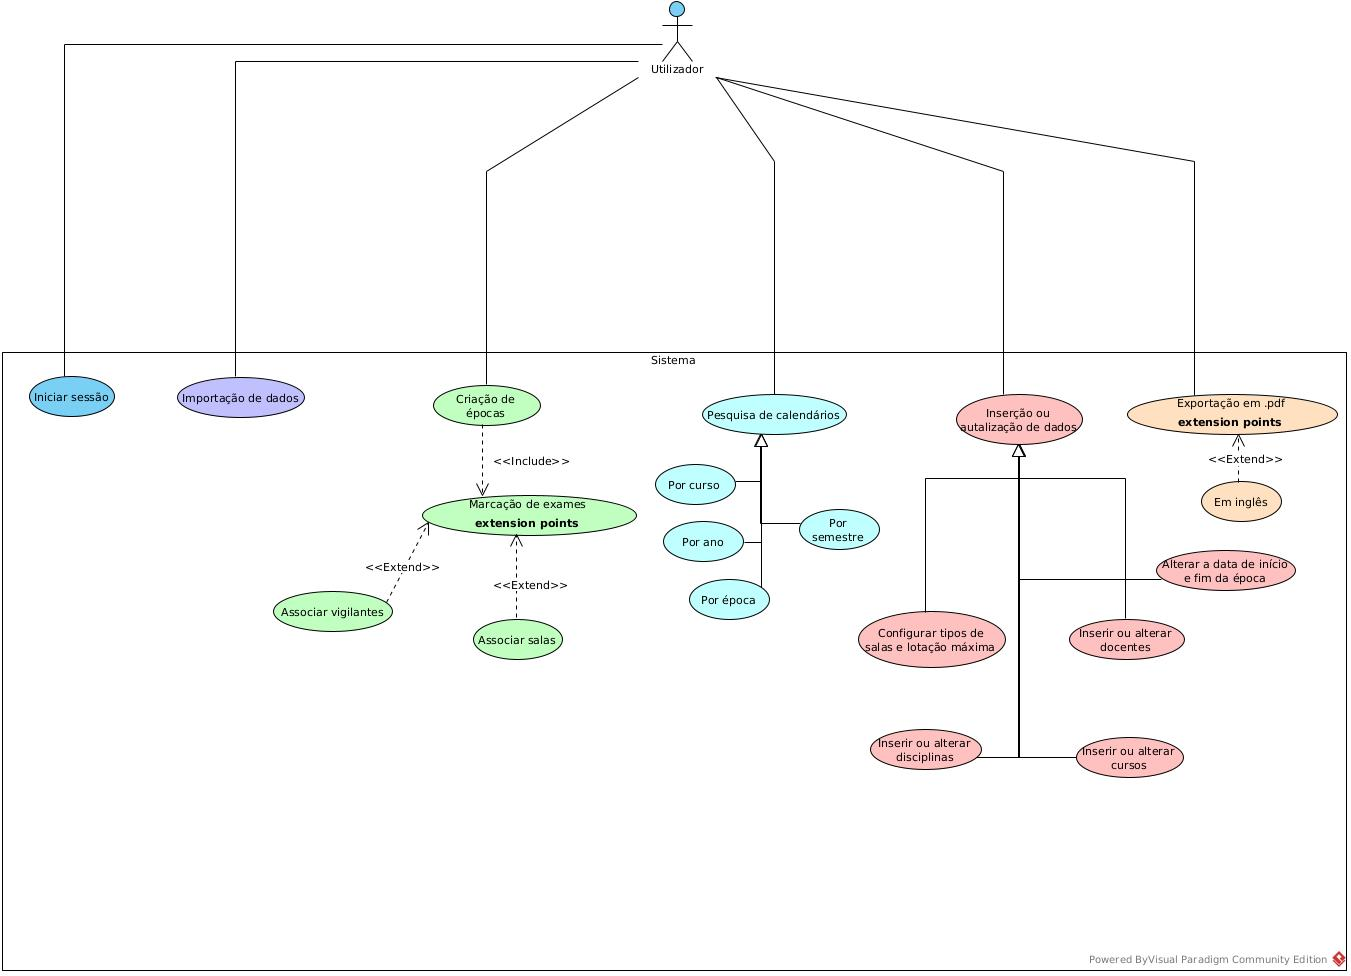
\includegraphics[width=1.3\textwidth,height=1.3\textheight,keepaspectratio]{image/diagrama}
			\caption{Diagrama dos casos de utilização}
		
		\end{figure}
\end{landscape}


	\section{Seleção dos casos de utilização}
	\label{selecaocasosdeuso}
	Os casos de utilização da primeira fase:
	
	\begin{itemize}
		\item Autenticação;
	 	\item Criação de épocas com data de início e fim;
	 	\item Configuração dos tipos de salas e a lotação máxima;
	 	\item Marcação de exames no calendário.
	 	\item Pesquisa de calendários por curso, ano, semestre e época de avaliação;
	\end{itemize}
	
	Segunda fase:
	\begin{itemize}
		\item Importação de ficheiros .csv com a configuração de salas, disciplinas e docentes;
		\item Inserção de cursos e disciplinas;
		\item Restringir a marcação de exames ao domingos e feriados;
		\item Associar um ou mais docentes aos exames para serem vigilantes;
		\item Inserção de novos docentes;
		\item Associar uma ou mais salas a um exame;
		\item Exportação do calendário em formato pdf;
	\end{itemize}


	Terceira fase:
	\begin{itemize}
		\item Associar na área de docentes dias em que os mesmos não estão disponíveis;
		\item Editar informações sobre os docentes;
		\item Avisar se houver sobreposição de exames;
		\item Avisar se o docente não estiver disponível;
		\item Avisar se houver mais alunos inscritos do que a lotação máxima da sala;
		\item Avisar se a sala não estiver disponível;
		\item Avisar caso o docente associado ao exame for repetido;
	\end{itemize}
	
	Quarta fase:
	\begin{itemize}
		\item Avisar se o curso for diurno e houver uma marcação para o turno da noite e vice-versa.
		\item Associar o mesmo exame a todos os cursos que têm a mesma disiplina.
		\item Avisar caso o tipo de sala associada ao exame não for apropriada (informática ou normal)
		\item Exportação do calendário em inglês
	\end{itemize}

	
	\section{Descrição dos casos de utilização}
	
	
		
	\begin{table}[H]
		\caption{Caso de utilização - autenticação}
		\begin{center}	
			\begin{tabularx}{\textwidth}{|l|X|}
				\hline
				\textbf{Nome }	& \textbf{Autenticação} \\
				\hline
				Atores: & Utilizador \\
				\hline
				Prioridade: & Alta \\
				\hline
				Requisitos funcionais:&  \\
				\hline
				Finalidade: & Aceder às funcionalidades da aplicação\\
				\hline
				Sumário: &  \\
				\hline
				Pré-condições: & Ter uma conta registada na aplicação e estar dentro da rede da UA\\
				\hline
				Descrição da interação: &  O utilizador assim que abre a aplicação tem de iniciar a sessão com o seu email e palavra-passe correspondentes\\
				\hline
				Cenário alternativo:&\\
				\hline
			\end{tabularx}
		\end{center}
	\end{table}

\begin{table}[H]
	\caption{Caso de utilização - criação de épocas de avaliação}
	\begin{center}	
		\begin{tabularx}{\textwidth}{|l|X|}
			\hline
			\textbf{Nome }	& \textbf{Criação de épocas de avaliação} \\
			\hline
			Atores: & Utilizador\\
			\hline
			Prioridade: &  Alta\\
			\hline
			Requisitos funcionais:&  \\
			\hline
			Finalidade: & Criação de épocas (com data de início e fim) para a realização de exames. \\
			\hline
			Sumário: & O utilizador pode criar épocas de exames para os vários cursos. Cada época estará associada a um ano, semestre e um nome dado pelo utilizador.\\
			\hline
			Pré-condições: & Ter iniciado sessão na aplicação.\\
			\hline
			Descrição da interação: &  \\
			\hline
			Cenário alternativo: &\\
			\hline
		\end{tabularx}
	\end{center}
\end{table}


\begin{table}[H]
	\caption{Caso de utilização - marcação de exames}
	\begin{center}	
		\begin{tabularx}{\textwidth}{|l|X|}
			\hline
			\textbf{Nome }	& \textbf{Marcação de exames} \\
			\hline
			Atores: & Utilizador\\
			\hline
			Prioridade: &  Alta\\
			\hline
			Requisitos funcionais:&  \\
			\hline
			Finalidade: & Marcação de exames na época de avaliações\\
			\hline
			Sumário: & O utilizador pode marcar os exames na época de avaliações escolhida. Pode marcar num dos três turnos: manhã, tarde e noite.\\
			\hline
			Pré-condições: & Ter iniciado sessão na aplicação, ter importado ou adicionado informações sobre os cursos, disciplinas, docentes e salas e ter escolhido o curso e a época de avaliações.\\
			\hline
			Descrição da interação: &  \\
			\hline
			Cenário alternativo: &\\
			\hline
		\end{tabularx}
	\end{center}
\end{table}


	
	

\begin{table}[H]
	\caption{Caso de utilização - pesquisa de calendários}
	\begin{center}	
		\begin{tabularx}{\textwidth}{|l|X|}
			\hline
			\textbf{Nome }	& \textbf{Pesquisa de calendários} \\
			\hline
			Atores: & Utilizador\\
			\hline
			Prioridade: &  Alta\\
			\hline
			Requisitos funcionais:&  \\
			\hline
			Finalidade: & Pesquisa de calendários através de filtros.\\
			\hline
			Sumário: & O utilizador pode pesquisar entre todos os calendários criados através de filtros como o curso, ano, semestre ou ano.\\
			\hline
			Pré-condições: & Ter iniciado sessão na aplicação e ter criado calendários de avaliação\\
			\hline
			Descrição da interação: &  \\
			\hline
			Cenário alternativo: &\\
			\hline
		\end{tabularx}
	\end{center}
\end{table}


	
	\chapter{Prototipagem}
	\section{Protótipo de baixa fidelidade}
	\subsection{Wireframes}
	\subsection{Diagrama de user flow}
	\subsection{Testes}
	\subsubsection{Análise de resultados}
	
	\section{Protótipo de alta fidelidade}
	\subsection{Desenvolvimento do protótipo}
	\subsection{Guia de estilos}
	\subsection{Testes}
	\subsubsection{Análise de resultados}
	
	\chapter{Implementação do modelo de dados persistentes}
	\section{Estrutura da base de dados}
	\subsection{Base de dados - factories}
	\section{Arquitetura do sistema - Modelo MVC}
	\subsection{Models e Controllers}
	
	\chapter{Primeira versão da aplicação}
	\section{Implementação de funcionalidades}
	
	\chapter{Testes finais}
	\section{Testes com potenciais clientes}
	\section{Testes de acessibilidade}
	\section{Análise de resultados}
	
	\chapter{Lançamento da versão final}
	\section{Alocação da aplicação no servidor}
	
	
	\chapter{Reflexão crítica e conclusão}
	
	

	\bibliographystyle{ieeetr}
	\bibliography{citations}
	
\end{document}	
	
	
	
	
